\documentclass[12pt, letterpaper]{article}
\renewcommand{\baselinestretch}{1.1}
\usepackage[english]{babel}
\usepackage[utf8]{inputenc}



\usepackage{amssymb}
\usepackage{mathtools}
\usepackage{hyperref}
\usepackage{amsmath}
\usepackage{float}
\usepackage{graphicx}
\usepackage{subfig}
\usepackage[table]{xcolor}
\usepackage[dvipsnames]{xcolor}

\usepackage{booktabs,tabularx}
\usepackage{booktabs,tabulary}

\usepackage[scale=1.0,left = 0.75in, right = 0.75in, ,top=0.8in,bottom=0.8in]{geometry}

\title{Automated Deployment of Machine Learning Benchmarkas on Hadoop MapReduce with HiBench}
\author{Ali Aaramesh}
\date{May 2016}

\begin{document}

\maketitle

\section{Introduction}
In this project we focused on automated deployment of Machine Learning benhcmarks of Intel corporations's comprehensive Hadoop benchmark suit, HiBench. \cite{hibench2} Deployment of large scale systems within virtual clusters provided by cloud infrastructure are non trivial system level tasks which constitute of many small steps to be done on every single machine in the cluster. Most of tehse tasks are the same for all machines, but you need to repeat them over all machines in the cluster. For example, if you install Java JDK on all your linux machines, you wll end up follwoing exactly the same steps on all machines. Therefore that would be great to be able to automate these tasks. Here in this project we do so by using Ansible which is one of the most sophisticated tools to automate apps and IT infrastructure, or so called DevOps tools. In simple terms, Ansible combines application deployment, configuration management, and continuous delivery.

The problem that we have chosen to work on to automate is about quantification of performance of Apache Hadoop implementation of MapReduce for machine learning workloads in terms of run time and throughput. There is no need to highlight the importance of doing such a project when we take a look at how Hadoop is becoming more and more influencial part of cloud computing infrastructures. With ongoing growth in using Hadoop in cloud infrastructures, it is a crucial step before deploying Hadoop to measure it's performance. Here we will use HiBench, a representative and comprehensive Hadoop benchmark suite developed at Intel \cite{hibench3} to test Hadoop's performance for typical machine learning tasks. This suit contains both micro-benchmarks and real-world programs. This project is aimed to focus on machine learning benchmarks included in HiBench. We should emphasize that the project's main goal is not to analyse the results of the benchmarks, but the to automate the process of running such benchmarks. 


\section{Machine Learning Benchmarks in HiBench}
HiBench's machine learning suit includes Bayesian Classification and K-means Clustering implementations contained in Apache Mahout which is an open-source  machine learning library built on top of Hadoop. These two well-known methods are representative of one important use case of MapReduce, that is large-scale machine learning.
As describet at \cite{hibench2} the Bayesian Classification workload implements the
trainer part of Naive Bayesian, that is where it extracts the terms
using the N-Gram algorithm from input web page text,
calculates the Tf-Idf for each term, and perform the weighting and
normalization. The input of Bayesian Classification is extracted from a
subset of the Wikipedia dump which is split and then prepared into text samples using the built-in
WikipediaXmlSplitter and WikipediaDatasetCreator in Mahout. The text samples are finally distributed into several files as the input of the benchmark.

The K-means Clustering workload implements K-means algorithm for clustering. 
Its input is a set of numerical vectorised samples. The workload first computes the centroid of each
cluster by running one Hadoop job iteratively, utill a convergence condition is satisfied or a maximum number of iterations is passed. Then a clustering job that
assigns each sample to a cluster runs to lable points with their cluster lable. K-means input in HiBench is generated based on a random data generator using statistic distributions.



\section{Implementation}

The technologies used in this project includes Apache Hadoop, Apache Spark, and Apache Mahout. Ansible is used to set-up the cluster envirnoment and deploy the benchmarks. There is no specific need for programming in this project, however, Python is used for visualisation of the results. Input datasets for the benchmarks will be generated at the runtime and we do not need to already have any dataset or database.


The implementation of teh project which basically is automoation of Hadoop benchmarking includes three major steps: 

\begin{itemize}
    \item Set up a virtual cluster
    \item Install basic packages, Hadoop, and Spark
    \item Install and run HiBench Machine Learning benchmarks
\end{itemize}

For the first and second steps we have relied on Big Data Analytics Stack \cite{bds} which is provided by researchers at the Indiana University Bloomington and includes comprehensive set of Ansble roles and playbooks to be used for big data analysis mostly over Apache infrastructure.  To install adn run the HiBench machine learning benchmarks we have developed many Ansible playbooks which can be found at \cite{hibenchconf}. When the deployment of the playbooks finishes successfully the rsults will be ploted for three differet easures: run time duration, throughput per node, and total throughput. 

\subsection{Issues}
Implementation of the project included many issues. To name a few I should refer, lack of support for issues in public communities like stackoverflow which makes it very tedious ro debug the deployment process. For example I had to debug the execution of the code by my self to find out that the linux dictionary words under $/usr/share/dict/words$ were not installed by default in the instances created by the Big Data Analytics Stack. In few cases I had to come up with my own way to include Hadoop configuration parameters in the HiBench configuration directory. For example HiBench does not support Hadoop Zookeeper based configuration and I had to manually (actually using Ansible tasks) extract cluster information like list of slave nodes.


\begin{figure}
\centering
\begin{tabular}{ccc}
\subfloat[Run time]{
  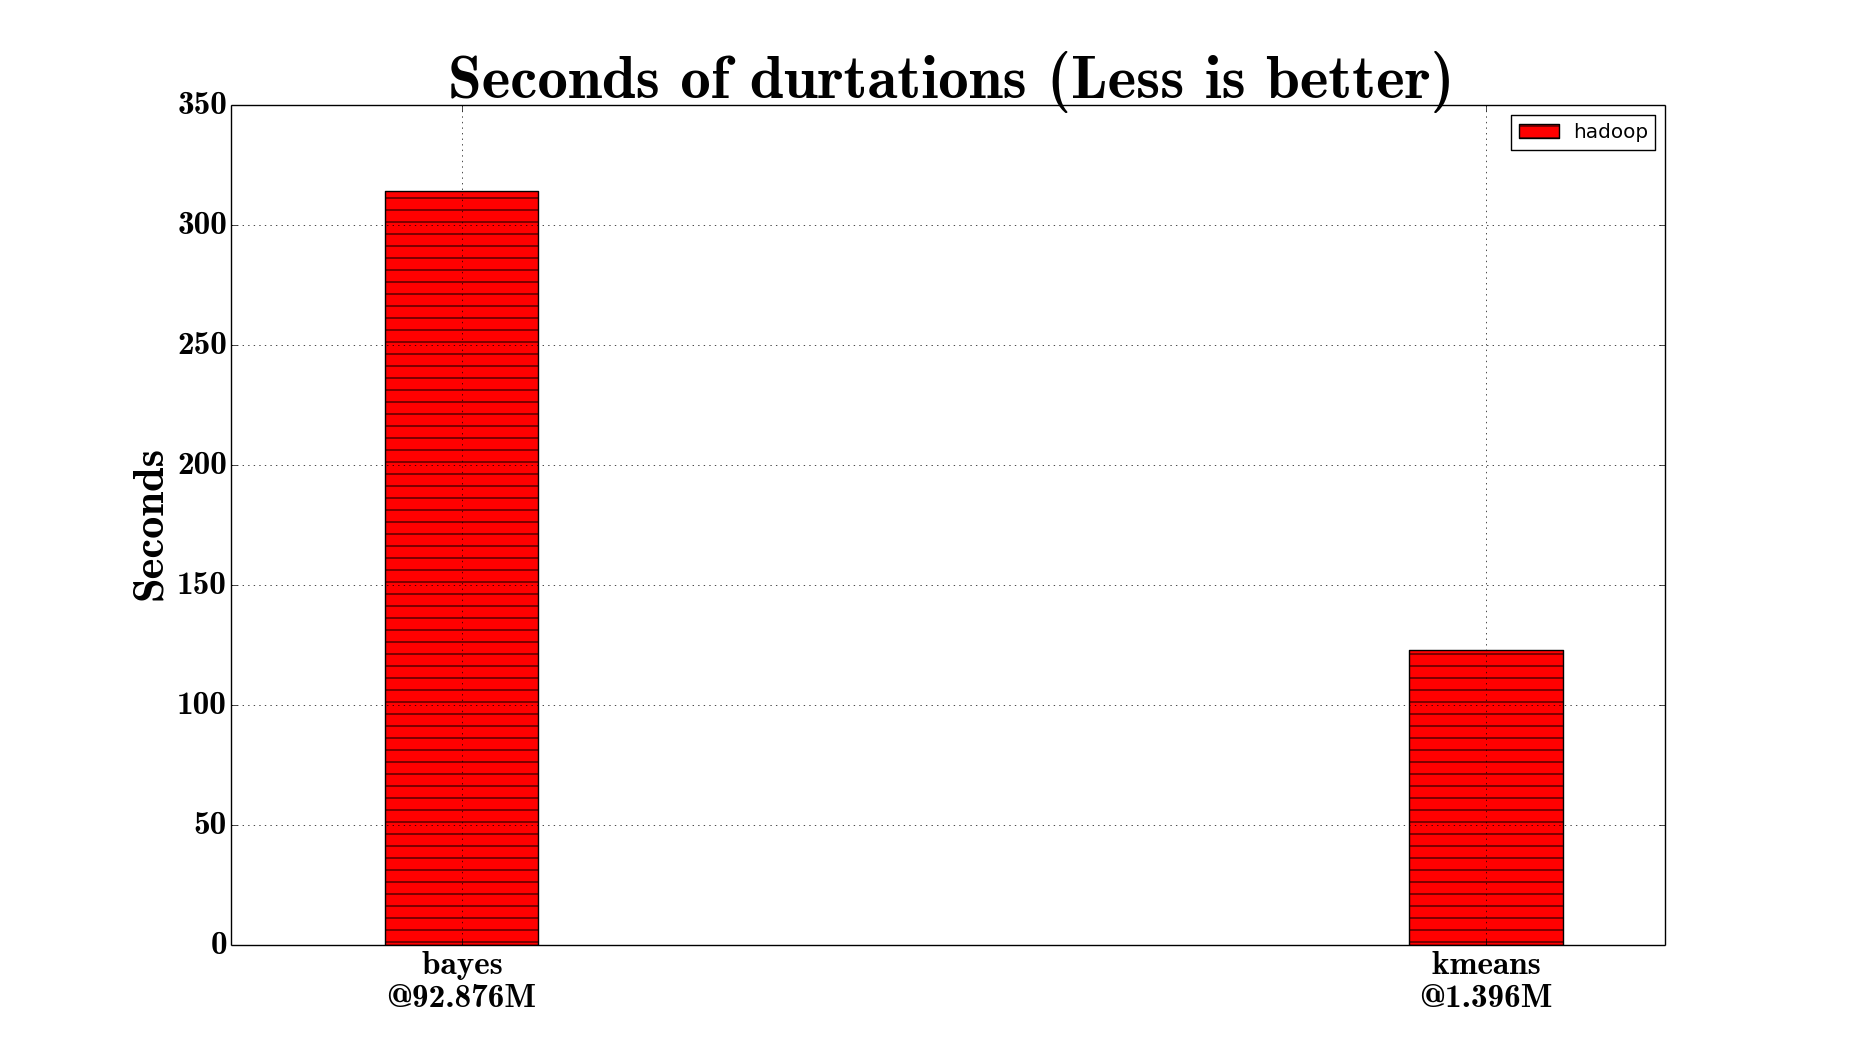
\includegraphics[width=70mm]{tiny/durtation.png}
}

\subfloat[Throughput per node]{
  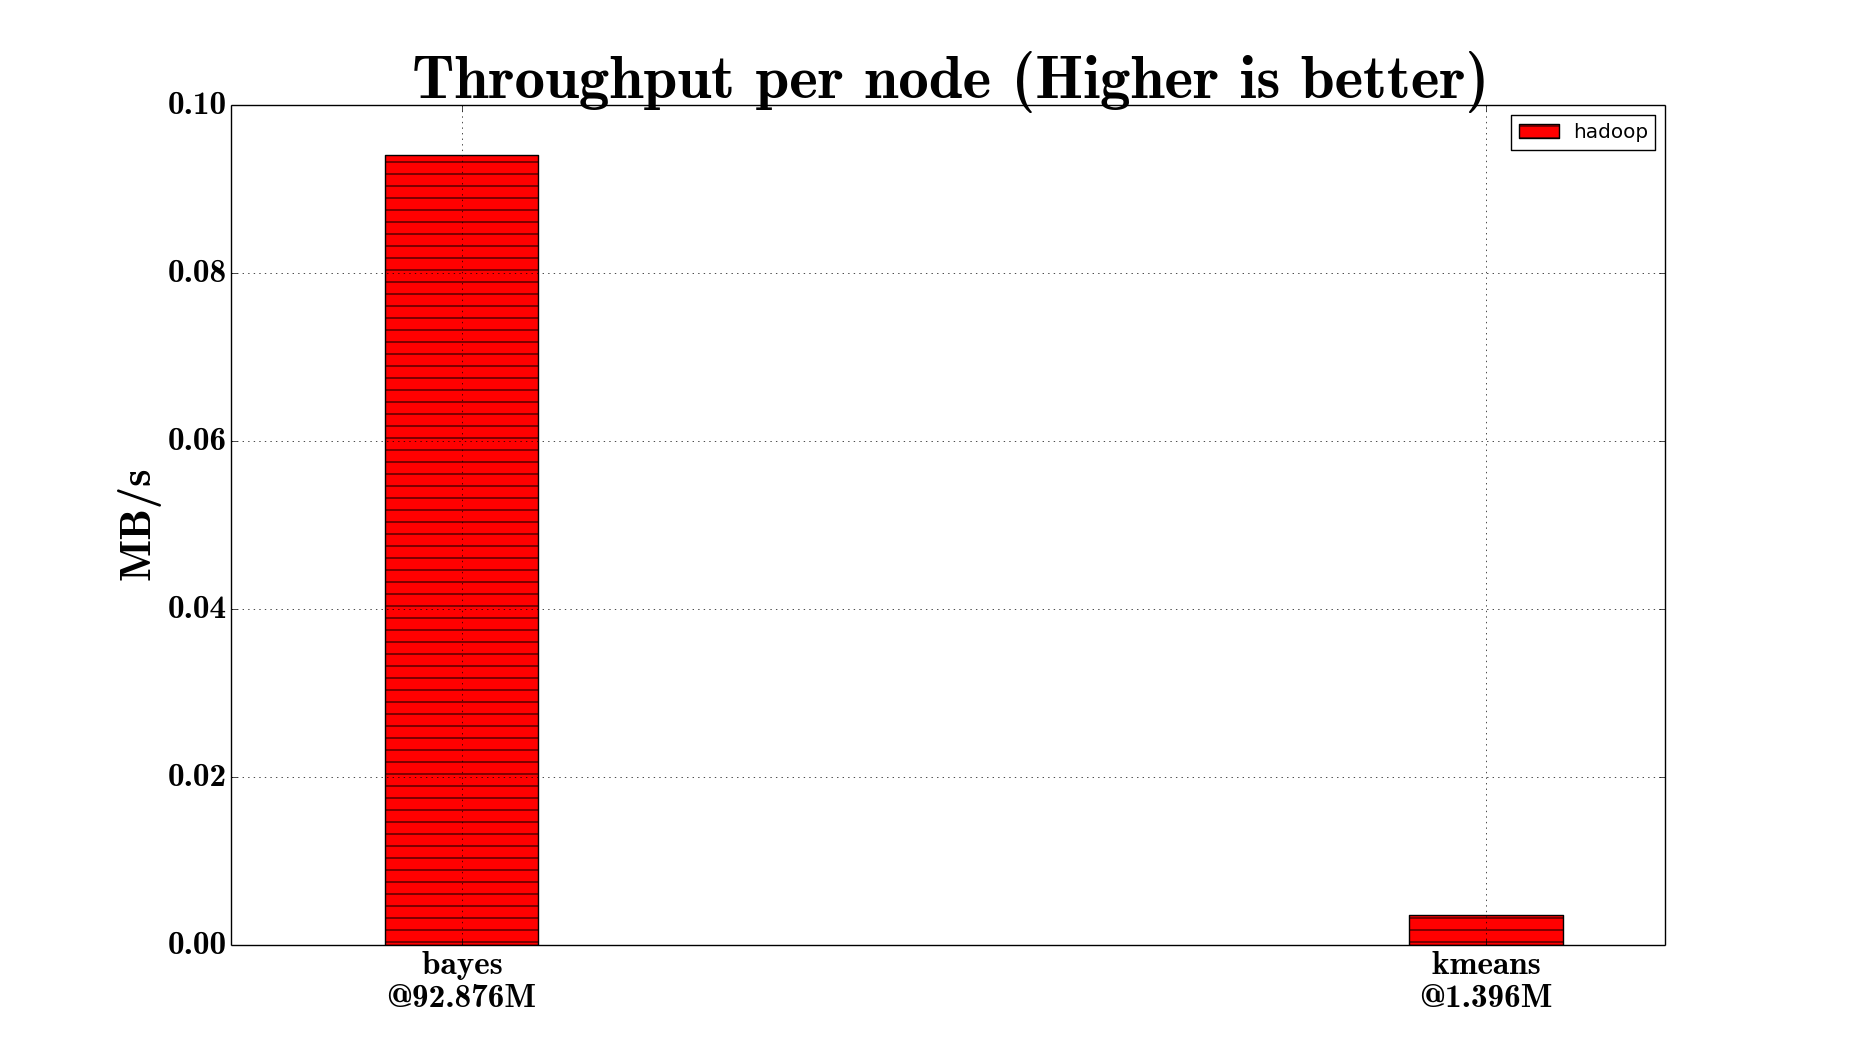
\includegraphics[width=70mm]{tiny/throughput_per_node.png}
}

\\

\subfloat[Total throughput]{
  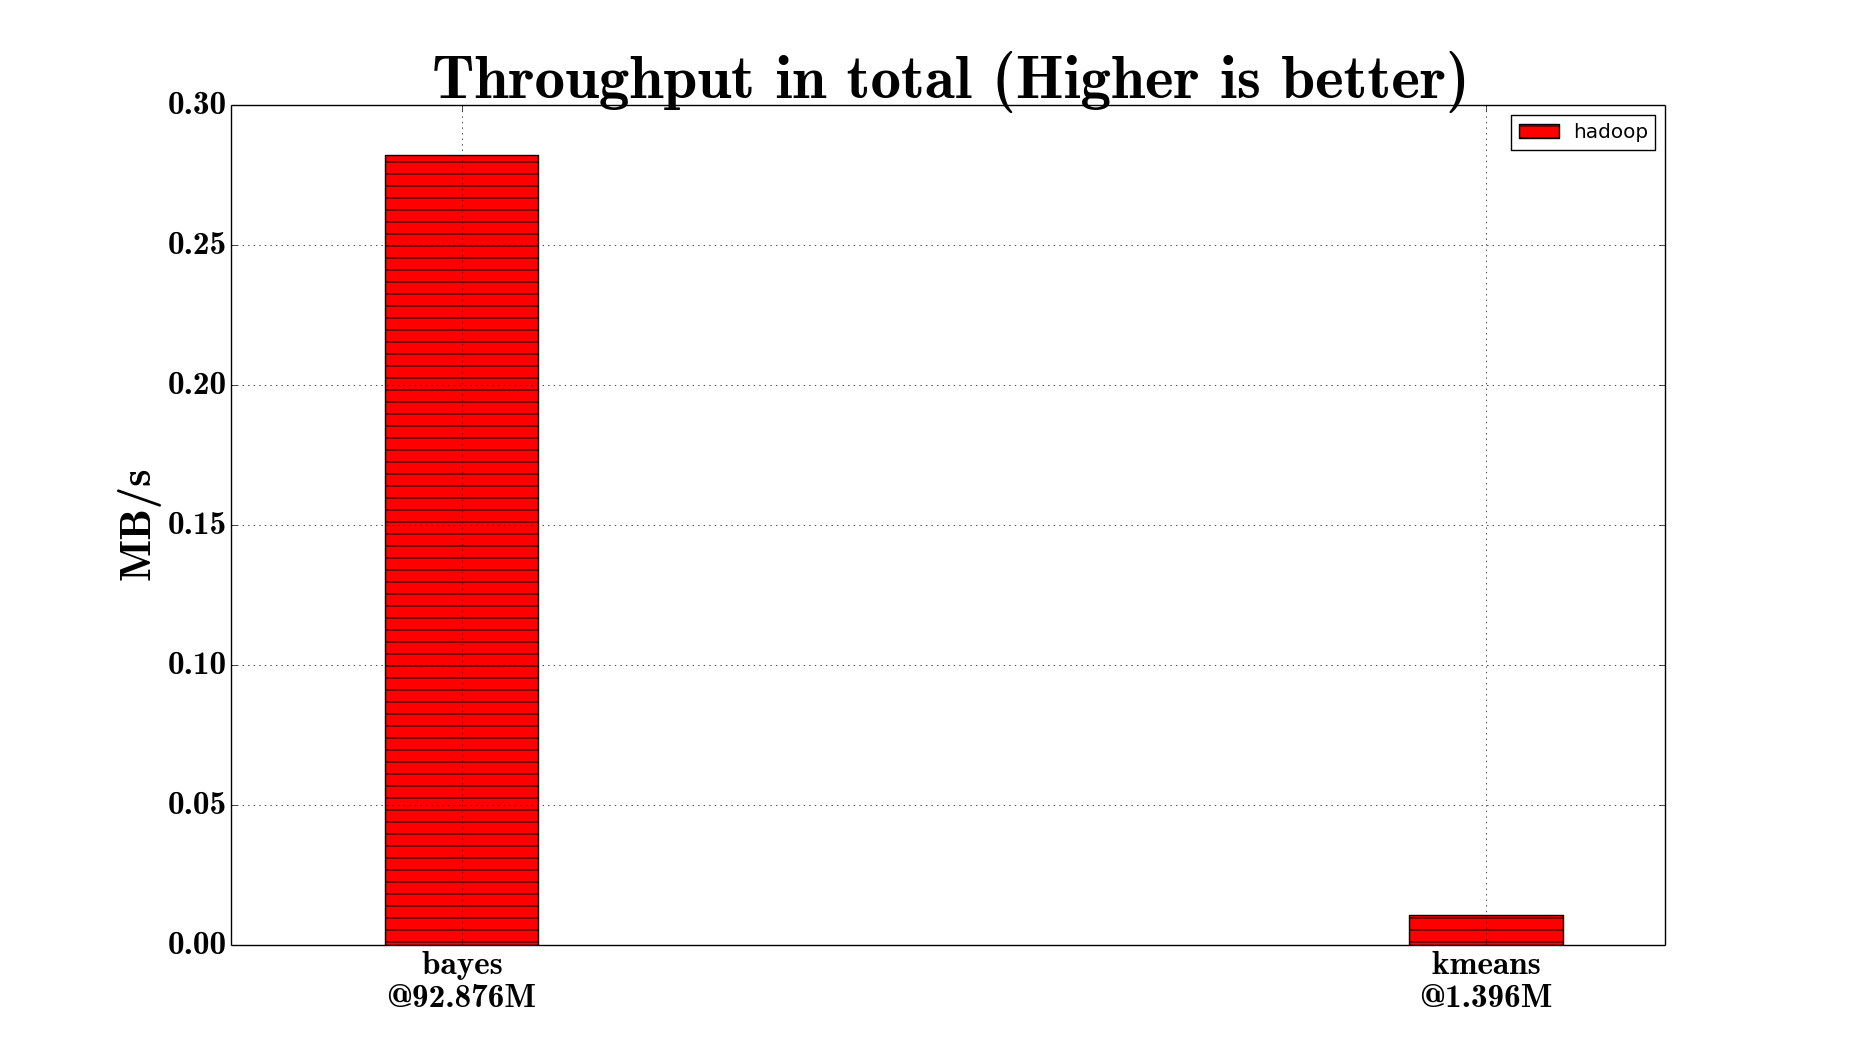
\includegraphics[width=70mm]{tiny/throughput_total.png}
}
\end{tabular}
\caption{Benchmarks results for Naive bayes classification and K-Means clustering algorithms for tiny scale workload.}
\label{tiny}
\end{figure}

\begin{figure}
\centering
\begin{tabular}{ccc}
\subfloat[Run time]{
  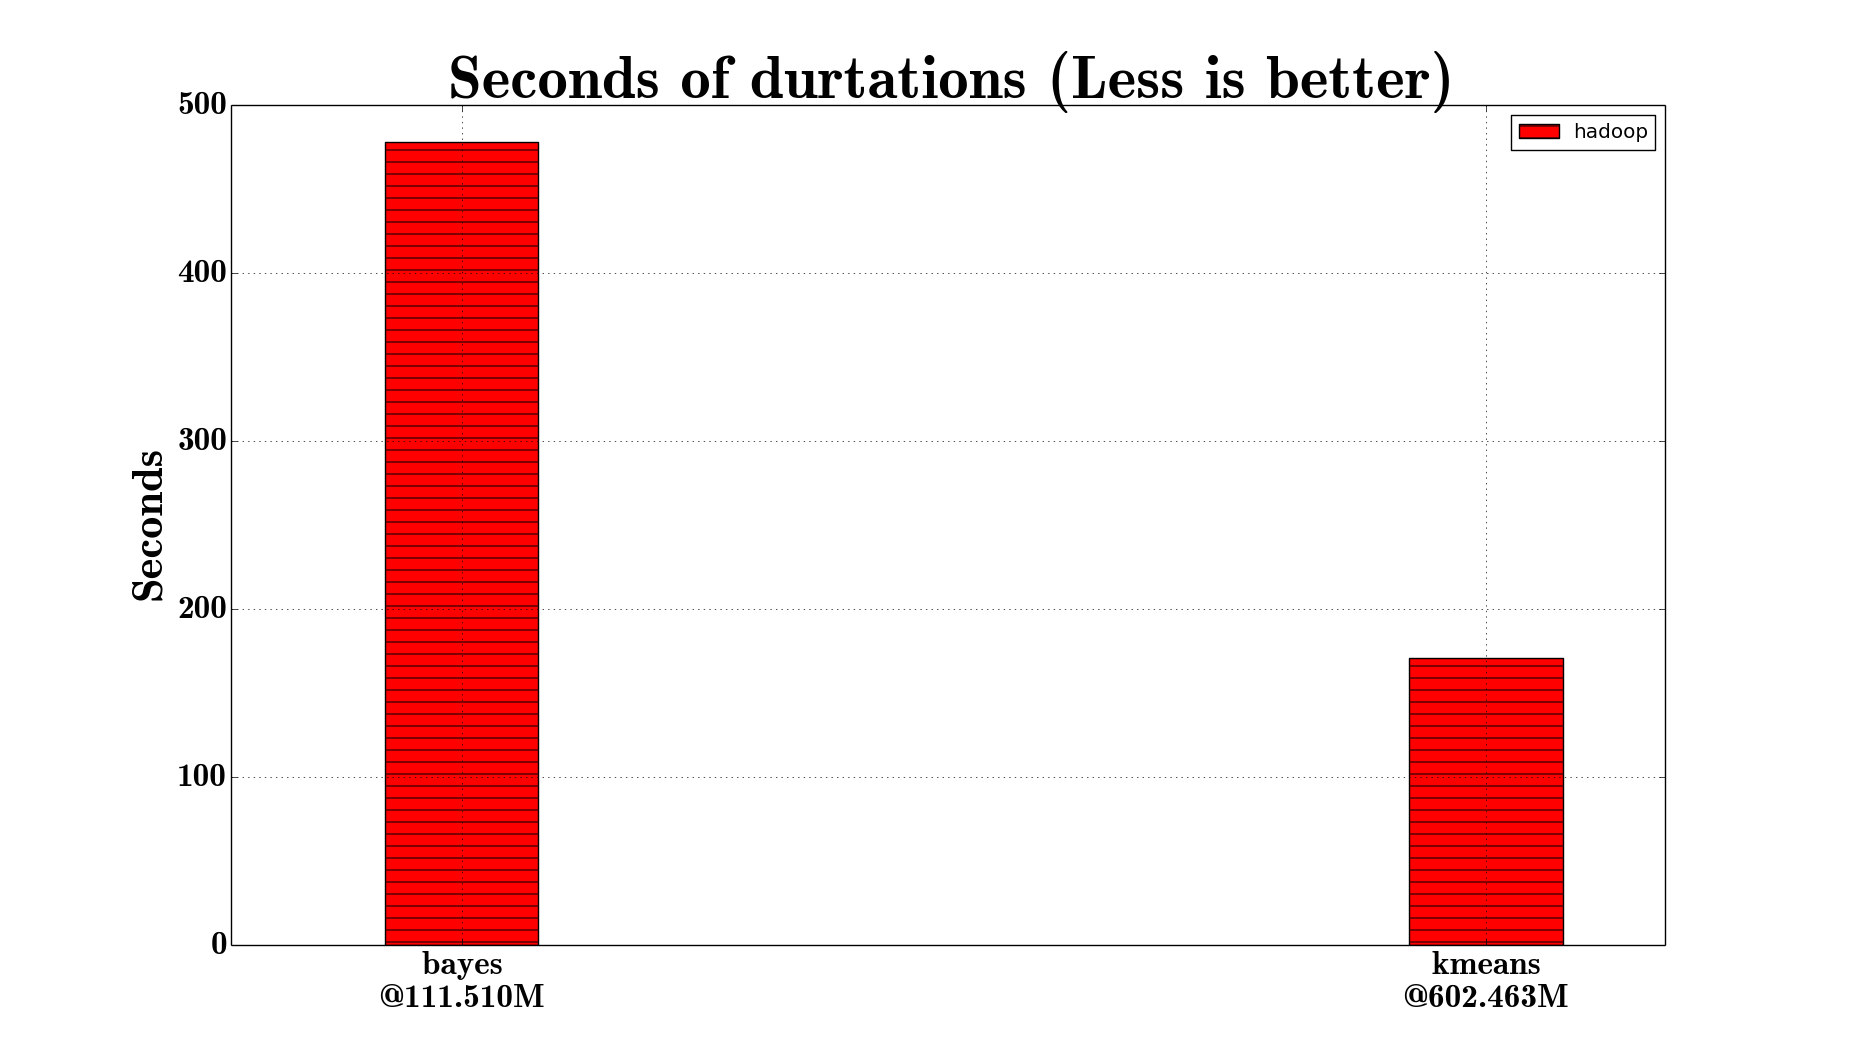
\includegraphics[width=70mm]{small/durtation.png}
}

\subfloat[Throughput per node]{
  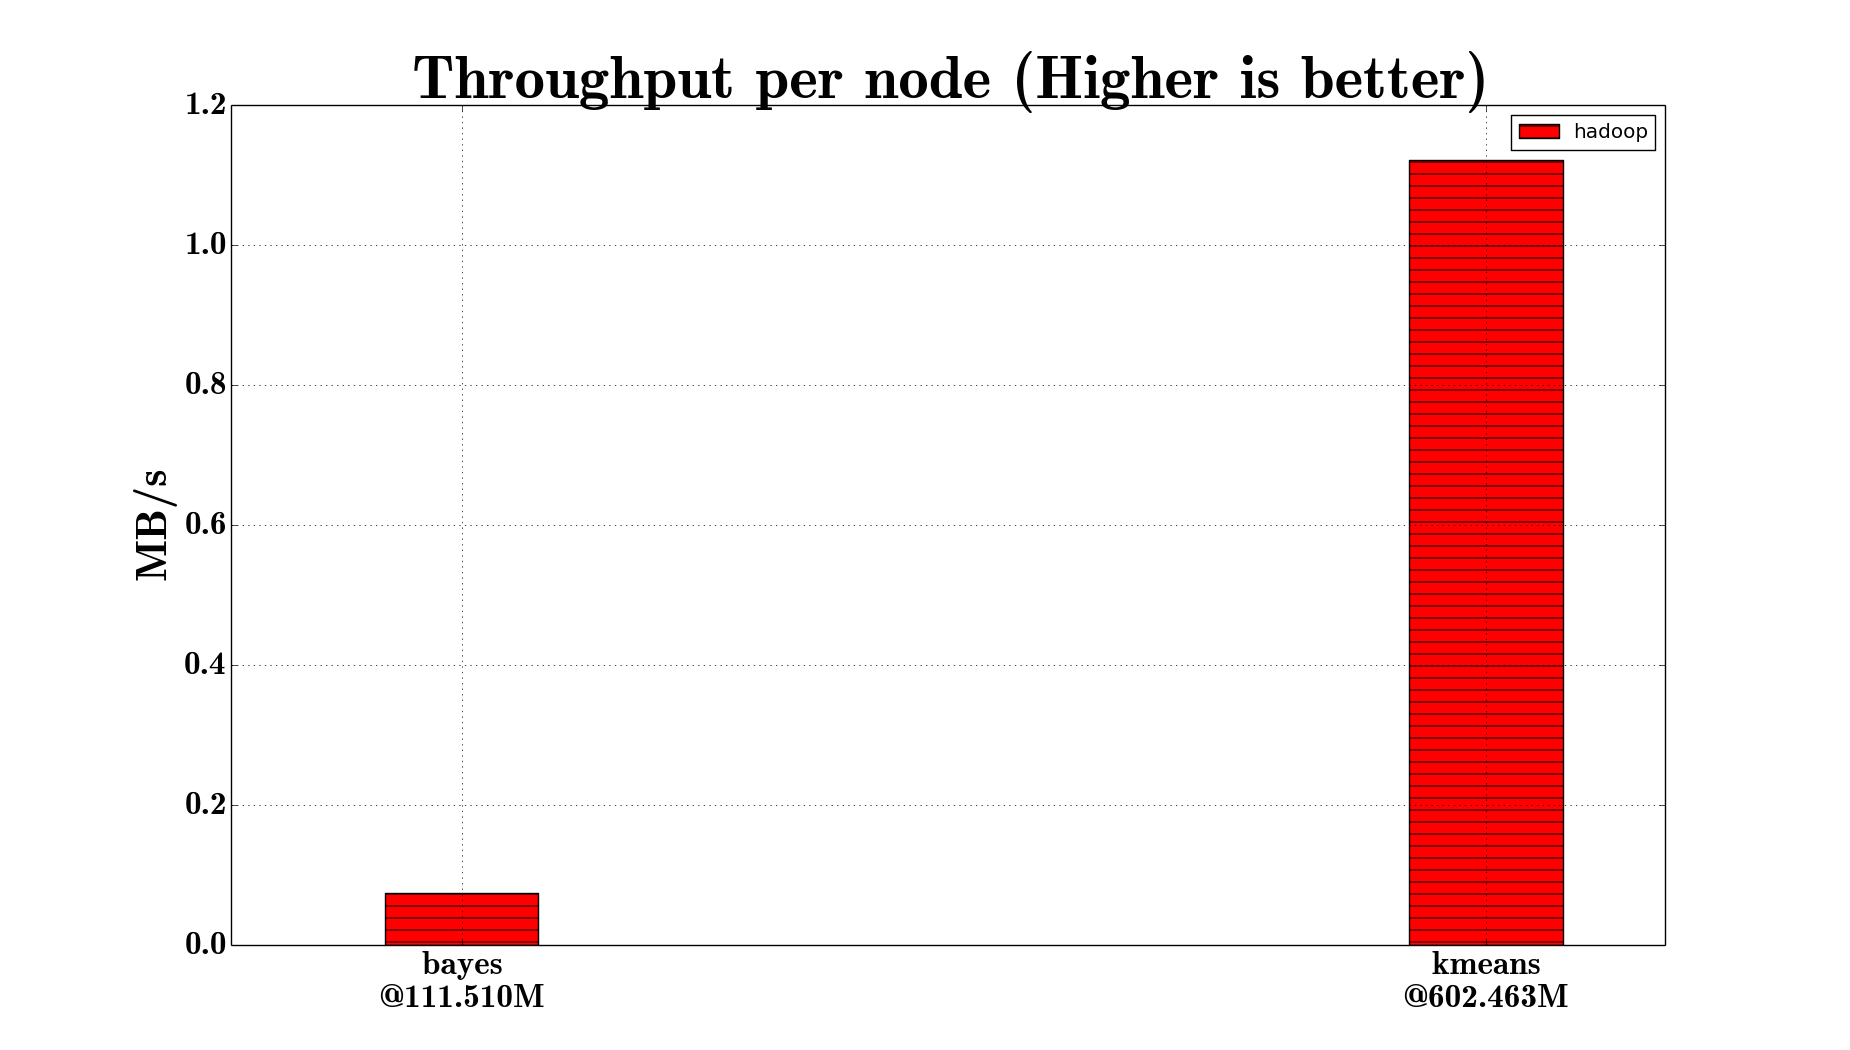
\includegraphics[width=70mm]{small/throughput_per_node.png}
}

\\

\subfloat[Total throughput]{
  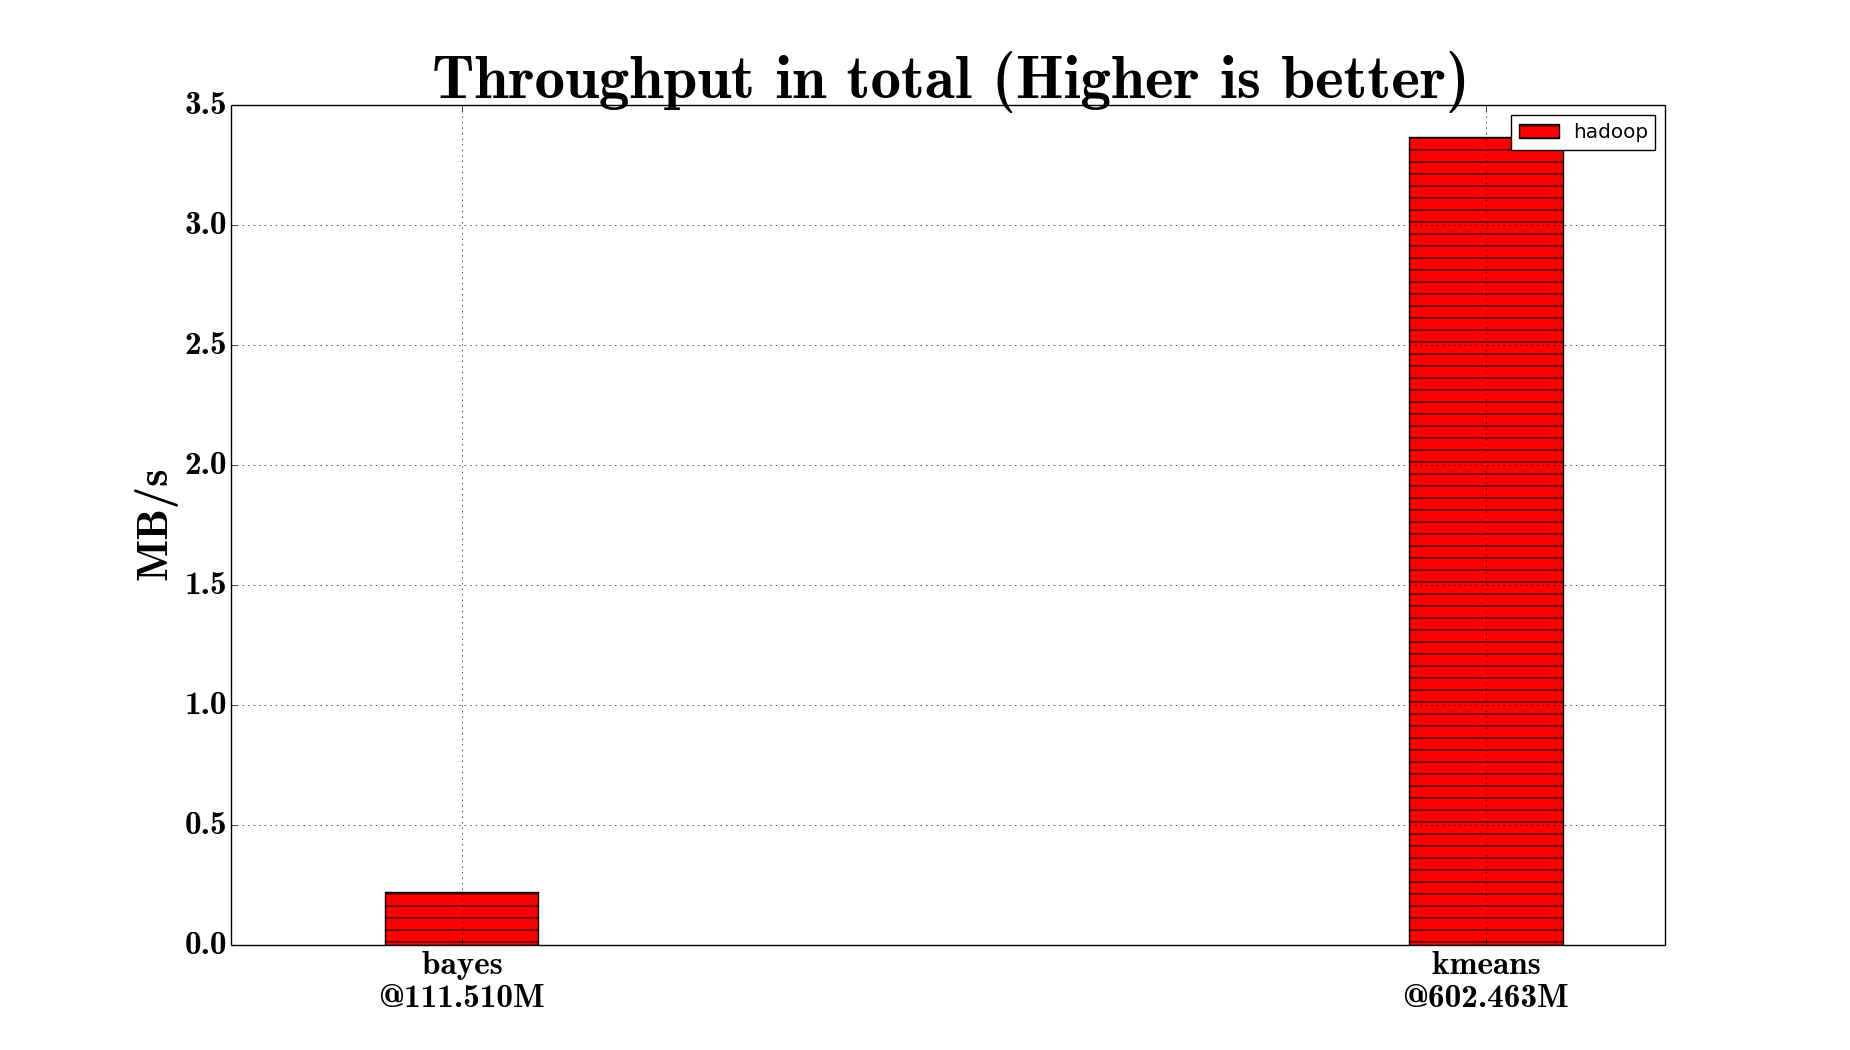
\includegraphics[width=70mm]{small/throughput_total.png}
}
\end{tabular}
\caption{Benchmarks results for Naive bayes classification and K-Means clustering algorithms for small scale workload.}
\label{small}
\end{figure}



\begin{figure}
\centering
\begin{tabular}{ccc}
\subfloat[Run time]{
  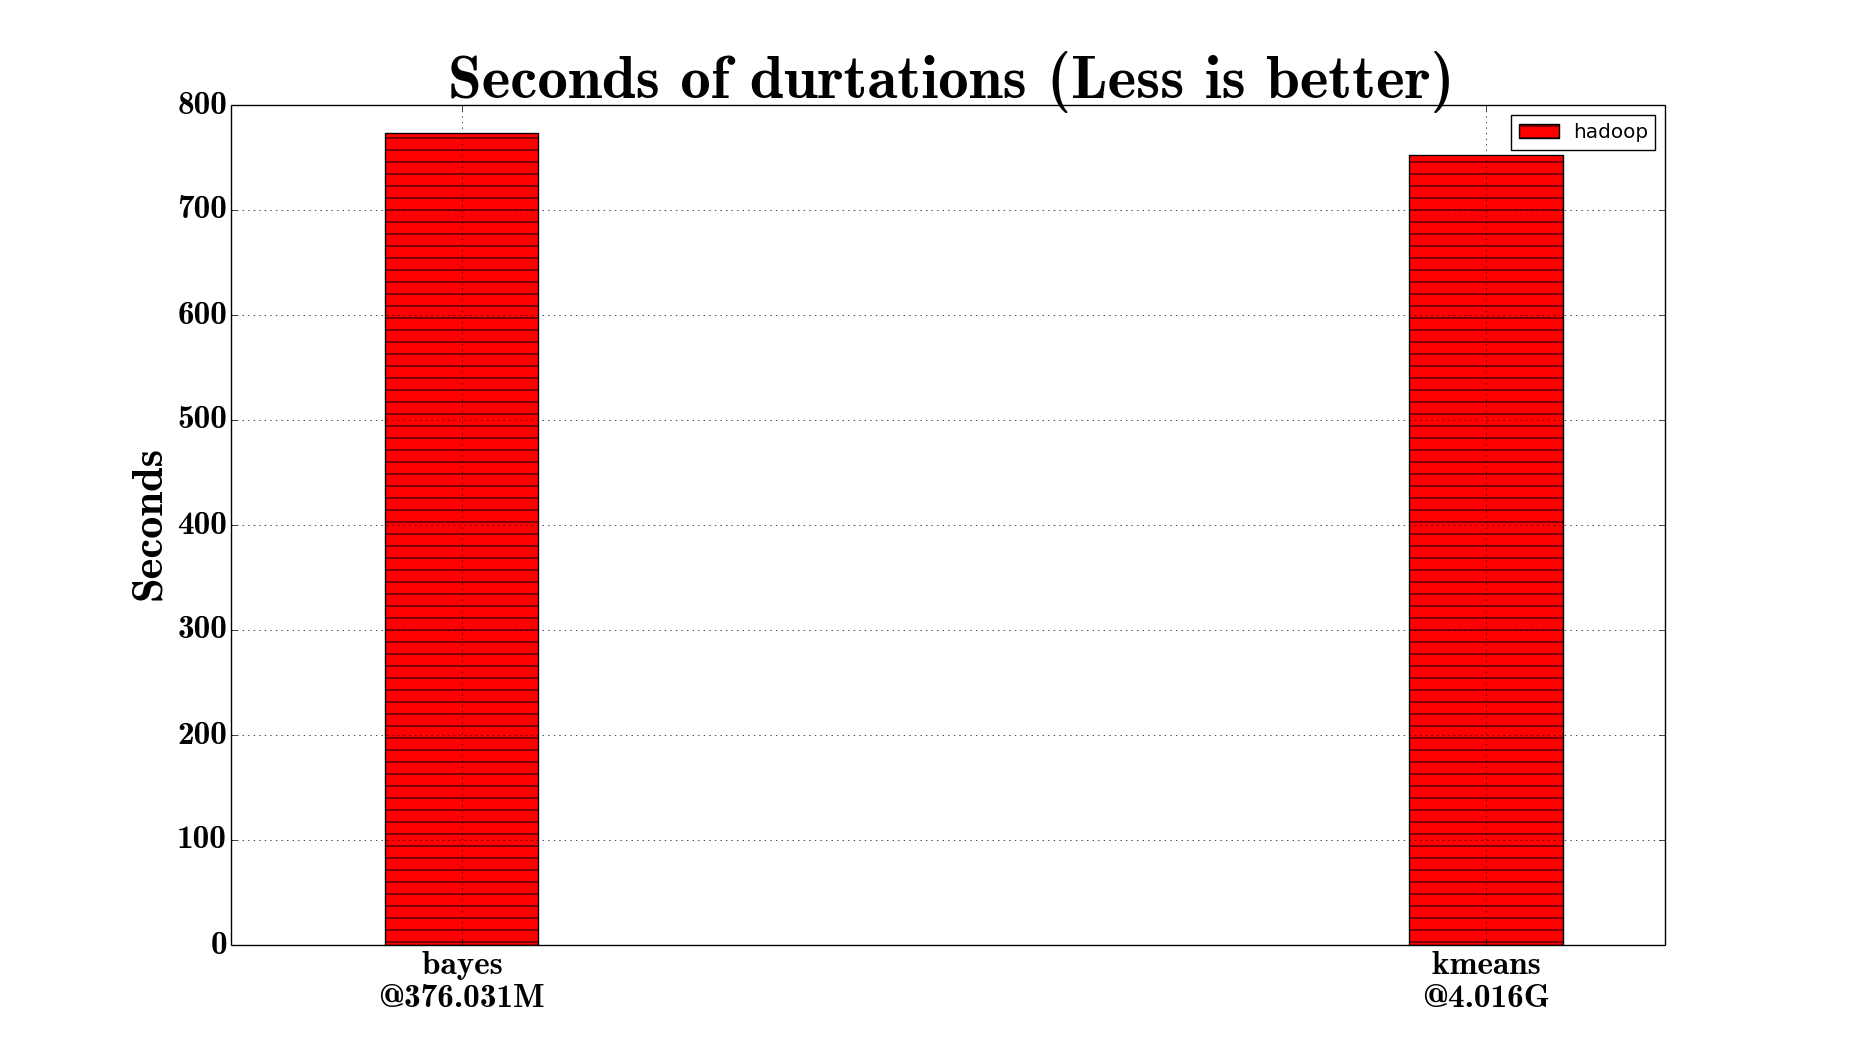
\includegraphics[width=70mm]{large/durtation.png}
}

\subfloat[Throughput per node]{
  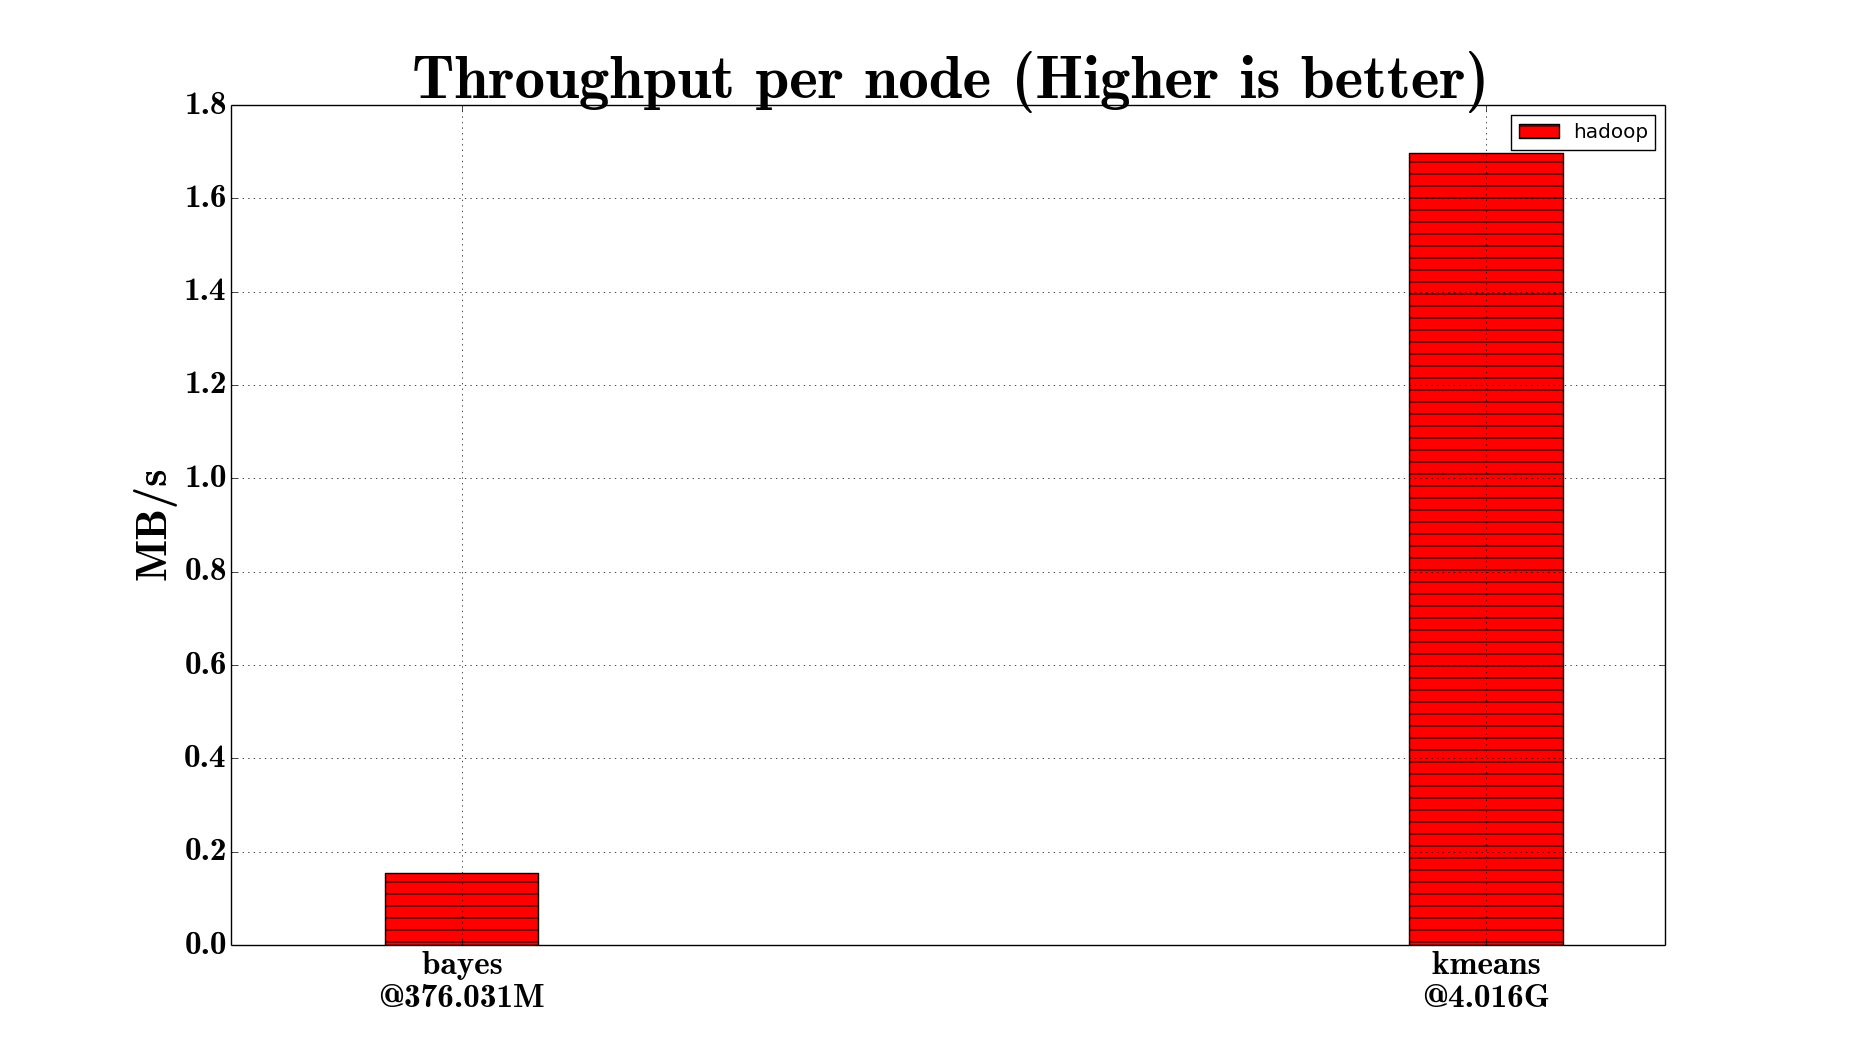
\includegraphics[width=70mm]{large/throughput_per_node.png}
}

\\

\subfloat[Total throughput]{
  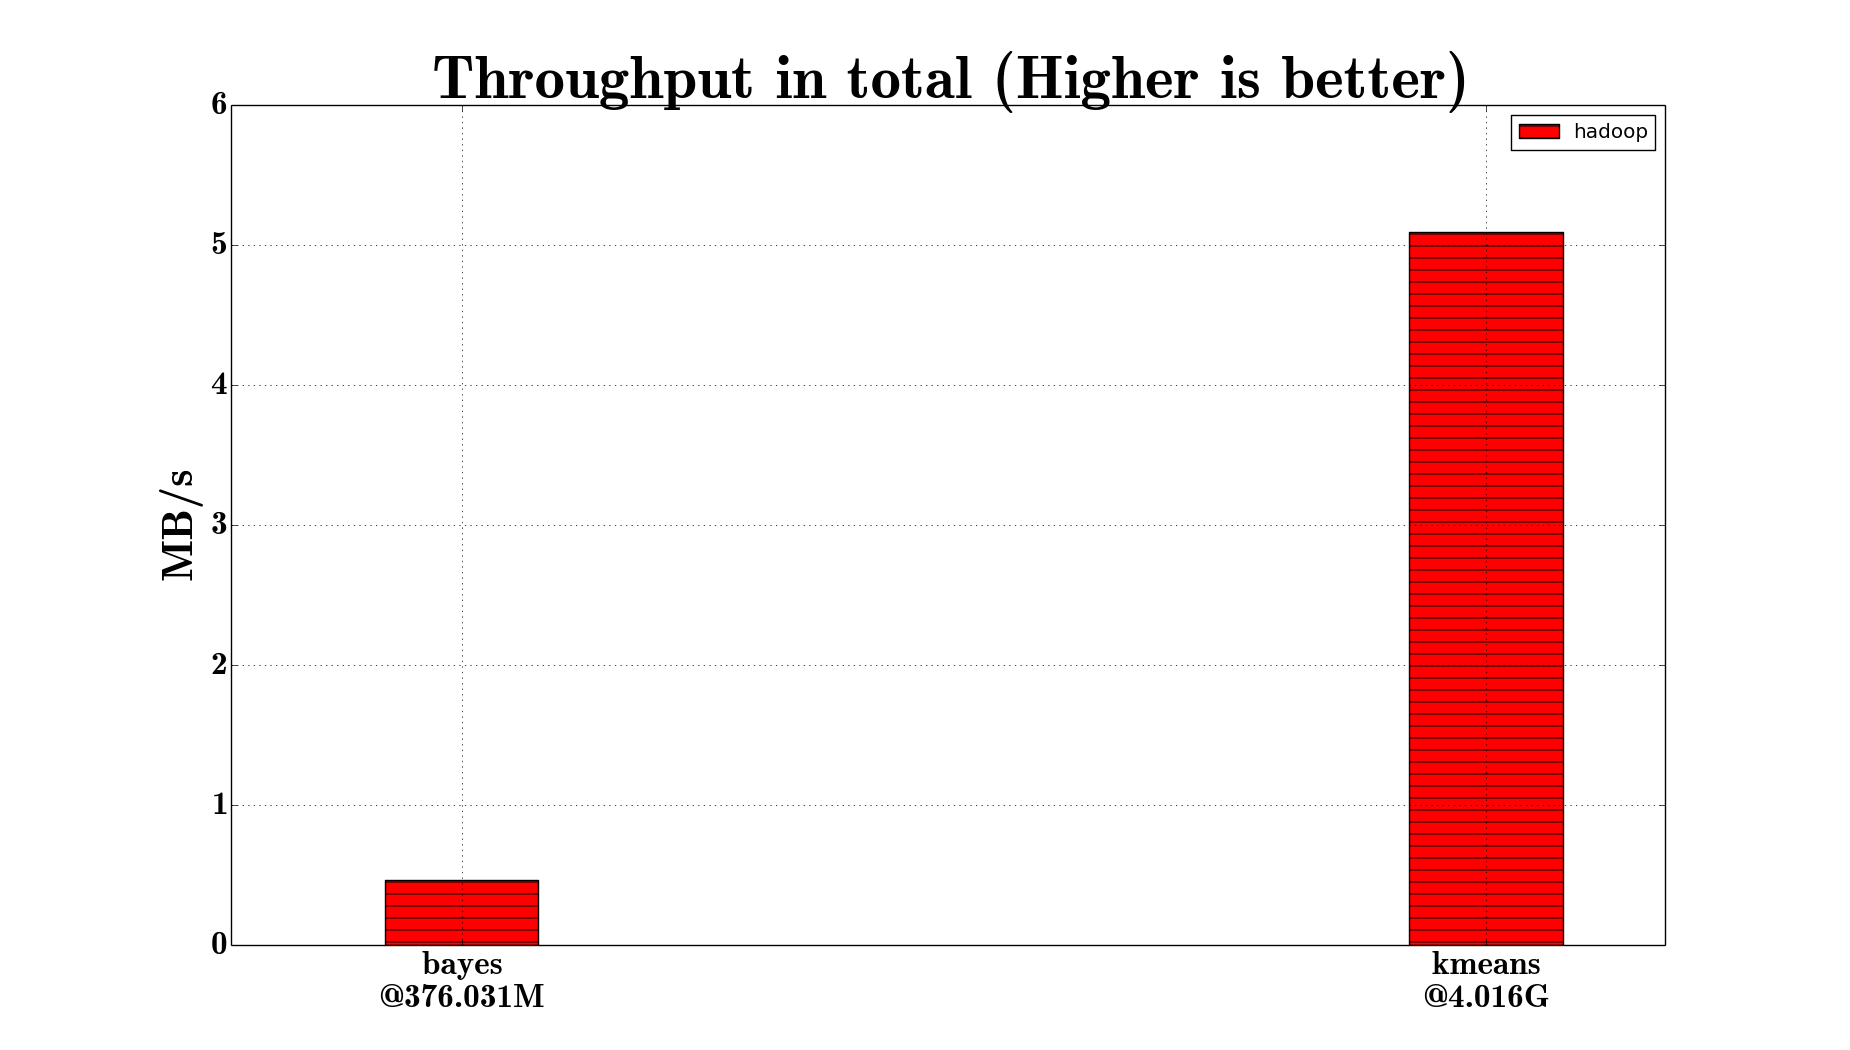
\includegraphics[width=70mm]{large/throughput_total.png}
}
\end{tabular}
\caption{Benchmarks results for Naive bayes classification and K-Means clustering algorithms for large scale workload.}
\label{large}
\end{figure}

\section{Benchmark Results}

HiBench defines some workload scales as input for Naive Bayes and K-Means algorithms. These predefined scales include tiny, small, large, huge, gigantic, and bigdata scales. For Naive Bayes, scales differbased on the number of pages to be classified, number of class lables, and length of n-grams. For K-Means each scale has seven parameters, number of true clusters, dimension of data points, number of data points, nummber of samples per input file, maximum number of iterations, k, and converging threshold. Detailed information about the values assigned for different scales can be found at \cite{hibenchconf}

Figures \ref{tiny}, \ref{small}, and \ref{large} show benchmark results for Naive Bayes classification and K-Means clustering algorithms for three different scales, tiny, small, and large respectively. For each of the three sclaes, three digrams show the run time perphormace of the execution, throughput per node and total throughput. 



\begin{thebibliography}{9}
\bibitem{hibench1} 
Shengsheng Huang et al. 
\textit{The HiBench benchmark suite: Characterization of the MapReduce-based data analysis}. 
New Frontiers in Information and Software as Services, Springer, 2011.
 
\bibitem{hibench2} 
Shengsheng Huang et al.
\textit{Hibench: A representative and comprehensive hadoop benchmark suite}.
Proc. ICDE Workshops, 2010.

\bibitem{bds}
\textit{Big Data Analytics Stack}
\url{https://github.com/futuresystems/big-data-stack}

\bibitem{hibenchml}
\textit{HiBench-ML: Automated deployment of Intel HiBench Machine Learning benchmarks}
\url{https://github.iu.edu/alivara/HiBench-ML}


\bibitem{hibench3}
\textit{HiBench Benchmarking Suite}
\url{https://github.com/intel-hadoop/HiBench/blob/a0ac3e44e83f819637db0a818c9da958e7046a9f/conf/10-data-scale-profile.conf}

\bibitem{hibenchconf}
\textit{HiBench parameter values for different scales}
\url{https://github.com/intel-hadoop/HiBench/blob/a0ac3e44e83f819637db0a818c9da958e7046a9f/conf/10-data-scale-profile.conf}

\end{document}



